\chapter{Xác suất (Probability)}

\index{probability}

Một \key{xác suất (probability)} là một số thực trong khoảng từ $0$ đến $1$
chỉ ra khả năng xảy ra của một biến cố.
Nếu một biến cố chắc chắn sẽ xảy ra,
xác suất của nó là 1,
và nếu một biến cố không thể xảy ra,
xác suất của nó là 0.
Xác suất của một biến cố được ký hiệu là $P(\cdots)$
trong đó ba dấu chấm mô tả biến cố đó.

Ví dụ, khi gieo một con súc sắc,
kết quả là một số nguyên từ $1$ đến $6$,
và xác suất của mỗi kết quả là $1/6$.
Ví dụ, chúng ta có thể tính các xác suất sau:

\begin{itemize}[noitemsep]
\item $P(\textrm{''kết quả là 4''})=1/6$
\item $P(\textrm{''kết quả không phải là 6''})=5/6$
\item $P(\textrm{''kết quả là số chẵn''})=1/2$
\end{itemize}

\section{Tính toán}

Để tính xác suất của một biến cố,
chúng ta có thể sử dụng tổ hợp
hoặc mô phỏng quá trình tạo ra biến cố đó.
Ví dụ, chúng ta hãy tính xác suất
rút được ba lá bài có cùng giá trị
từ một bộ bài đã được xáo trộn
(ví dụ, $\spadesuit 8$, $\clubsuit 8$ và $\diamondsuit 8$).

\subsubsection*{Phương pháp 1}

Chúng ta có thể tính xác suất bằng công thức

\[\frac{\textrm{số kết quả mong muốn}}{\textrm{tổng số kết quả}}.\]

Trong bài toán này, các kết quả mong muốn là những
trường hợp mà giá trị của mỗi lá bài là như nhau.
Có $13 {4 \choose 3}$ kết quả như vậy,
bởi vì có $13$ khả năng cho giá trị
của các lá bài và ${4 \choose 3}$ cách để
chọn $3$ chất từ $4$ chất có thể.

Tổng cộng có ${52 \choose 3}$ kết quả,
bởi vì chúng ta chọn 3 lá bài từ 52 lá.
Do đó, xác suất của biến cố là

\[\frac{13 {4 \choose 3}}{{52 \choose 3}} = \frac{1}{425}.\]

\subsubsection*{Phương pháp 2}

Một cách khác để tính xác suất là
mô phỏng quá trình tạo ra biến cố.
Trong ví dụ này, chúng ta rút ba lá bài, vì vậy quá trình
bao gồm ba bước.
Chúng ta yêu cầu mỗi bước của quá trình đều phải thành công.

Việc rút lá bài đầu tiên chắc chắn thành công,
vì không có ràng buộc nào.
Bước thứ hai thành công với xác suất $3/51$,
vì còn lại 51 lá bài và 3 trong số đó
có cùng giá trị với lá bài đầu tiên.
Tương tự, bước thứ ba thành công với xác suất $2/50$.

Xác suất để toàn bộ quá trình thành công là

\[1 \cdot \frac{3}{51} \cdot \frac{2}{50} = \frac{1}{425}.\]

\section{Biến cố (Events)}

Một biến cố trong lý thuyết xác suất có thể được biểu diễn dưới dạng một tập hợp
\[A \subset X,\]
trong đó $X$ chứa tất cả các kết quả có thể xảy ra
và $A$ là một tập hợp con các kết quả.
Ví dụ, khi gieo một con súc sắc, các kết quả là
\[X = \{1,2,3,4,5,6\}.\]
Bây giờ, ví dụ, biến cố ''kết quả là số chẵn''
tương ứng với tập hợp
\[A = \{2,4,6\}.\]

Mỗi kết quả $x$ được gán một xác suất $p(x)$.
Khi đó, xác suất $P(A)$ của một biến cố
$A$ có thể được tính bằng tổng
các xác suất của các kết quả bằng công thức
\[P(A) = \sum_{x \in A} p(x).\]
Ví dụ, khi gieo một con súc sắc,
$p(x)=1/6$ cho mỗi kết quả $x$,
vì vậy xác suất của biến cố
''kết quả là số chẵn'' là
\[p(2)+p(4)+p(6)=1/2.\]

Tổng xác suất của các kết quả trong $X$ phải
là 1, tức là, $P(X)=1$.

Vì các biến cố trong lý thuyết xác suất là các tập hợp,
chúng ta có thể thao tác với chúng bằng các phép toán tập hợp tiêu chuẩn:

\begin{itemize}
\item \key{Phần bù (complement)} $\bar A$ có nghĩa là
''$A$ không xảy ra''.
Ví dụ, khi gieo một con súc sắc,
phần bù của $A=\{2,4,6\}$ là
$\bar A = \{1,3,5\}$.
\item \key{Hợp (union)} $A \cup B$ có nghĩa là
''$A$ hoặc $B$ xảy ra''.
Ví dụ, hợp của
$A=\{2,5\}$
và $B=\{4,5,6\}$ là
$A \cup B = \{2,4,5,6\}$.
\item \key{Giao (intersection)} $A \cap B$ có nghĩa là
''$A$ và $B$ xảy ra''.
Ví dụ, giao của
$A=\{2,5\}$ và $B=\{4,5,6\}$ là
$A \cap B = \{5\}$.
\end{itemize}

\subsubsection{Phần bù}

Xác suất của phần bù
$\bar A$ được tính bằng công thức
\[P(\bar A)=1-P(A).\]

Đôi khi, chúng ta có thể giải quyết một bài toán dễ dàng
bằng cách sử dụng phần bù bằng cách giải bài toán ngược lại.
Ví dụ, xác suất nhận được
ít nhất một mặt sáu khi gieo súc sắc mười lần là
\[1-(5/6)^{10}.\]

Ở đây $5/6$ là xác suất mà kết quả
của một lần gieo không phải là sáu, và
$(5/6)^{10}$ là xác suất mà không có lần nào trong
mười lần gieo là sáu.
Phần bù của điều này là câu trả lời cho bài toán.

\subsubsection{Hợp}

Xác suất của hợp $A \cup B$
được tính bằng công thức
\[P(A \cup B)=P(A)+P(B)-P(A \cap B).\]
Ví dụ, khi gieo một con súc sắc,
hợp của các biến cố
\[A=\textrm{''kết quả là số chẵn''}\]
và
\[B=\textrm{''kết quả nhỏ hơn 4''}\]
là
\[A \cup B=\textrm{''kết quả là số chẵn hoặc nhỏ hơn 4''},\]
và xác suất của nó là
\[P(A \cup B) = P(A)+P(B)-P(A \cap B)=1/2+1/2-1/6=5/6.\]

Nếu các biến cố $A$ và $B$ là \key{rời nhau (disjoint)}, tức là,
$A \cap B$ là tập rỗng,
xác suất của biến cố $A \cup B$ đơn giản là

\[P(A \cup B)=P(A)+P(B).\]

\subsubsection{Conditional probability}

\index{conditional probability}

\key{Xác suất có điều kiện (conditional probability)}
\[P(A | B) = \frac{P(A \cap B)}{P(B)}\]
là xác suất của $A$
giả sử rằng $B$ xảy ra.
Do đó, khi tính
xác suất của $A$, chúng ta chỉ xem xét các kết quả
cũng thuộc về $B$.

Sử dụng các tập hợp trước đó,
\[P(A | B)= 1/3,\]
bởi vì các kết quả của $B$ là
$\{1,2,3\}$, và một trong số đó là chẵn.
Đây là xác suất của một kết quả chẵn
nếu chúng ta biết rằng kết quả nằm trong khoảng $1 \ldots 3$.

\subsubsection{Giao}

\index{independence}

Sử dụng xác suất có điều kiện,
xác suất của giao
$A \cap B$ có thể được tính bằng công thức
\[P(A \cap B)=P(A)P(B|A).\]
Các biến cố $A$ và $B$ là \key{độc lập (independent)} nếu
\[P(A|B)=P(A) \hspace{10px}\textrm{và}\hspace{10px} P(B|A)=P(B),\]
điều này có nghĩa là việc $B$ xảy ra không
thay đổi xác suất của $A$, và ngược lại.
Trong trường hợp này, xác suất của giao là
\[P(A \cap B)=P(A)P(B).\]
Ví dụ, khi rút một lá bài từ bộ bài, các biến cố
\[A = \textrm{''chất là chuồn''}\]
và
\[B = \textrm{''giá trị là bốn''}\]
là độc lập. Do đó biến cố
\[A \cap B = \textrm{''lá bài là bốn chuồn''}\]
xảy ra với xác suất
\[P(A \cap B)=P(A)P(B)=1/4 \cdot 1/13 = 1/52.\]

\section{Biến ngẫu nhiên (Random variables)}

\index{random variable}

Một \key{biến ngẫu nhiên (random variable)} là một giá trị được tạo ra
bởi một quá trình ngẫu nhiên.
Ví dụ, khi gieo hai con súc sắc,
một biến ngẫu nhiên có thể là
\[X=\textrm{''tổng của các kết quả''}.\]
Ví dụ, nếu các kết quả là $[4,6]$
(nghĩa là chúng ta gieo được mặt bốn trước rồi đến mặt sáu),
thì giá trị của $X$ là 10.

Chúng ta ký hiệu $P(X=x)$ là xác suất mà
giá trị của một biến ngẫu nhiên $X$ là $x$.
Ví dụ, khi gieo hai con súc sắc,
$P(X=10)=3/36$,
bởi vì tổng số kết quả là 36
và có ba cách có thể để có được
tổng 10: $[4,6]$, $[5,5]$ và $[6,4]$.

\subsubsection{Giá trị kỳ vọng (Expected value)}

\index{expected value}

\key{Giá trị kỳ vọng (expected value)} $E[X]$ chỉ ra
giá trị trung bình của một biến ngẫu nhiên $X$.
Giá trị kỳ vọng có thể được tính bằng tổng
\[\sum_x P(X=x)x,\]
trong đó $x$ duyệt qua tất cả các giá trị có thể của $X$.

Ví dụ, khi gieo một con súc sắc,
kết quả kỳ vọng là
\[1/6 \cdot 1 + 1/6 \cdot 2 + 1/6 \cdot 3 + 1/6 \cdot 4 + 1/6 \cdot 5 + 1/6 \cdot 6 = 7/2.\]

Một thuộc tính hữu ích của giá trị kỳ vọng là \key{tính tuyến tính (linearity)}.
Nó có nghĩa là tổng
$E[X_1+X_2+\cdots+X_n]$
luôn bằng tổng
$E[X_1]+E[X_2]+\cdots+E[X_n]$.
Công thức này đúng ngay cả khi các biến ngẫu nhiên
phụ thuộc vào nhau.

Ví dụ, khi gieo hai con súc sắc,
tổng kỳ vọng là
\[E[X_1+X_2]=E[X_1]+E[X_2]=7/2+7/2=7.\]

Bây giờ chúng ta hãy xem xét một bài toán trong đó
$n$ quả bóng được đặt ngẫu nhiên vào $n$ hộp,
và nhiệm vụ của chúng ta là tính
số hộp rỗng kỳ vọng.
Mỗi quả bóng có xác suất bằng nhau để
được đặt vào bất kỳ hộp nào.
Ví dụ, nếu $n=2$, các khả năng
như sau:
\begin{center}
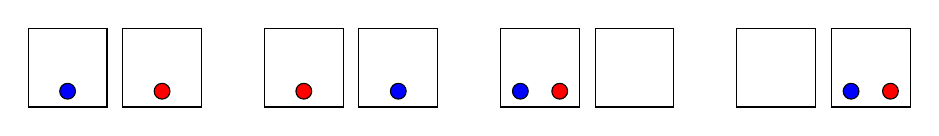
\begin{tikzpicture}
\draw (0,0) rectangle (1,1);
\draw (1.2,0) rectangle (2.2,1);
\draw (3,0) rectangle (4,1);
\draw (4.2,0) rectangle (5.2,1);
\draw (6,0) rectangle (7,1);
\draw (7.2,0) rectangle (8.2,1);
\draw (9,0) rectangle (10,1);
\draw (10.2,0) rectangle (11.2,1);

\draw[fill=blue] (0.5,0.2) circle (0.1);
\draw[fill=red] (1.7,0.2) circle (0.1);
\draw[fill=red] (3.5,0.2) circle (0.1);
\draw[fill=blue] (4.7,0.2) circle (0.1);
\draw[fill=blue] (6.25,0.2) circle (0.1);
\draw[fill=red] (6.75,0.2) circle (0.1);
\draw[fill=blue] (10.45,0.2) circle (0.1);
\draw[fill=red] (10.95,0.2) circle (0.1);
\end{tikzpicture}
\end{center}
Trong trường hợp này, số hộp rỗng
kỳ vọng là
\[\frac{0+0+1+1}{4} = \frac{1}{2}.\]
Trong trường hợp tổng quát, xác suất để một
hộp cụ thể bị rỗng là
\[\Big(\frac{n-1}{n}\Big)^n,\]
bởi vì không có quả bóng nào được đặt vào đó.
Do đó, sử dụng tính tuyến tính, số hộp rỗng
kỳ vọng là
\[n \cdot \Big(\frac{n-1}{n}\Big)^n.\]

\subsubsection{Phân phối (Distributions)}

\index{distribution}

\key{Phân phối (distribution)} của một biến ngẫu nhiên $X$
cho thấy xác suất của mỗi giá trị mà
$X$ có thể có.
Phân phối bao gồm các giá trị $P(X=x)$.
Ví dụ, khi gieo hai con súc sắc,
phân phối cho tổng của chúng là:
\begin{center}
\small {
\begin{tabular}{r|rrrrrrrrrrrrr}
$x$ & 2 & 3 & 4 & 5 & 6 & 7 & 8 & 9 & 10 & 11 & 12 \\
$P(X=x)$ & $1/36$ & $2/36$ & $3/36$ & $4/36$ & $5/36$ & $6/36$ & $5/36$ & $4/36$ & $3/36$ & $2/36$ & $1/36$ \\
\end{tabular}
}
\end{center}

\index{uniform distribution}
Trong một \key{phân phối đều (uniform distribution)},
biến ngẫu nhiên $X$ có $n$ giá trị có thể
$a,a+1,\ldots,b$ và xác suất của mỗi giá trị là $1/n$.
Ví dụ, khi gieo một con súc sắc,
$a=1$, $b=6$ và $P(X=x)=1/6$ cho mỗi giá trị $x$.

Giá trị kỳ vọng của $X$ trong phân phối đều là
\[E[X] = \frac{a+b}{2}.\]

\index{binomial distribution}
Trong một \key{phân phối nhị thức (binomial distribution)}, $n$ lần thử
được thực hiện
và xác suất để một lần thử thành công
là $p$.
Biến ngẫu nhiên $X$ đếm số lần
thử thành công,
và xác suất của một giá trị $x$ là
\[P(X=x)=p^x (1-p)^{n-x} {n \choose x},\]
trong đó $p^x$ và $(1-p)^{n-x}$ tương ứng với
các lần thử thành công và không thành công,
và ${n \choose x}$ là số cách
chúng ta có thể chọn thứ tự của các lần thử.

Ví dụ, khi gieo một con súc sắc mười lần,
xác suất gieo được mặt sáu đúng
ba lần là $(1/6)^3 (5/6)^7 {10 \choose 3}$.

Giá trị kỳ vọng của $X$ trong phân phối nhị thức là
\[E[X] = pn.\]

\index{geometric distribution}
Trong một \key{phân phối hình học (geometric distribution)},
xác suất để một lần thử thành công là $p$,
và chúng ta tiếp tục cho đến khi lần thành công đầu tiên xảy ra.
Biến ngẫu nhiên $X$ đếm số lần
thử cần thiết, và xác suất của
một giá trị $x$ là
\[P(X=x)=(1-p)^{x-1} p,\]
trong đó $(1-p)^{x-1}$ tương ứng với các lần thử không thành công
và $p$ tương ứng với lần thử thành công đầu tiên.

Ví dụ, nếu chúng ta gieo một con súc sắc cho đến khi gieo được mặt sáu,
xác suất để số lần gieo
đúng bằng 4 là $(5/6)^3 1/6$.

Giá trị kỳ vọng của $X$ trong phân phối hình học là
\[E[X]=\frac{1}{p}.\]

\section{Chuỗi Markov (Markov chains)}

\index{Markov chain}

Một \key{chuỗi Markov (Markov chain)}
là một quá trình ngẫu nhiên
bao gồm các trạng thái và các chuyển tiếp giữa chúng.
Đối với mỗi trạng thái, chúng ta biết xác suất
để di chuyển đến các trạng thái khác.
Một chuỗi Markov có thể được biểu diễn dưới dạng một đồ thị
có các nút là trạng thái và các cạnh là các chuyển tiếp.

Ví dụ, hãy xem xét một bài toán
trong đó chúng ta đang ở tầng 1 của một tòa nhà $n$ tầng.
Ở mỗi bước, chúng ta ngẫu nhiên đi lên một tầng
hoặc đi xuống một tầng, ngoại trừ việc chúng ta luôn
đi lên một tầng từ tầng 1 và đi xuống một tầng
từ tầng $n$.
Xác suất ở tầng $m$
sau $k$ bước là bao nhiêu?

Trong bài toán này, mỗi tầng của tòa nhà
tương ứng với một trạng thái trong một chuỗi Markov.
Ví dụ, nếu $n=5$, đồ thị như sau:

\begin{center}
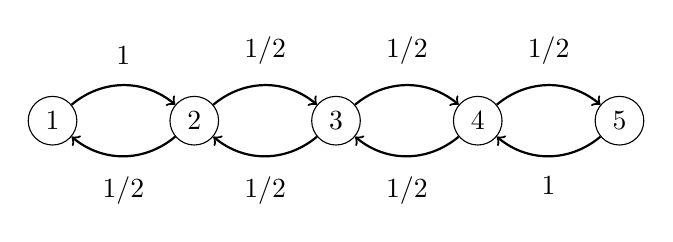
\begin{tikzpicture}[scale=0.9]
\node[draw, circle] (1) at (0,0) {$1$};
\node[draw, circle] (2) at (2,0) {$2$};
\node[draw, circle] (3) at (4,0) {$3$};
\node[draw, circle] (4) at (6,0) {$4$};
\node[draw, circle] (5) at (8,0) {$5$};

\path[draw,thick,->] (1) edge [bend left=40] node[font=\small,label=$1$] {} (2);
\path[draw,thick,->] (2) edge [bend left=40] node[font=\small,label=$1/2$] {} (3);
\path[draw,thick,->] (3) edge [bend left=40] node[font=\small,label=$1/2$] {} (4);
\path[draw,thick,->] (4) edge [bend left=40] node[font=\small,label=$1/2$] {} (5);

\path[draw,thick,->] (5) edge [bend left=40] node[font=\small,label=below:$1$] {} (4);
\path[draw,thick,->] (4) edge [bend left=40] node[font=\small,label=below:$1/2$] {} (3);
\path[draw,thick,->] (3) edge [bend left=40] node[font=\small,label=below:$1/2$] {} (2);
\path[draw,thick,->] (2) edge [bend left=40] node[font=\small,label=below:$1/2$] {} (1);

\end{tikzpicture}
\end{center}

Phân phối xác suất
của một chuỗi Markov là một vector
$[p_1,p_2,\ldots,p_n]$, trong đó $p_k$ là
xác suất mà trạng thái hiện tại là $k$.
Công thức $p_1+p_2+\cdots+p_n=1$ luôn đúng.

Trong kịch bản trên, phân phối ban đầu là
$[1,0,0,0,0]$, vì chúng ta luôn bắt đầu ở tầng 1.
Phân phối tiếp theo là $[0,1,0,0,0]$,
vì chúng ta chỉ có thể di chuyển từ tầng 1 đến tầng 2.
Sau đó, chúng ta có thể đi lên một tầng
hoặc đi xuống một tầng, vì vậy phân phối tiếp theo là
$[1/2,0,1/2,0,0]$, và cứ thế.

Một cách hiệu quả để mô phỏng việc di chuyển trong
một chuỗi Markov là sử dụng quy hoạch động.
Ý tưởng là duy trì phân phối xác suất,
và ở mỗi bước duyệt qua tất cả các khả năng
chúng ta có thể di chuyển.
Sử dụng phương pháp này, chúng ta có thể mô phỏng
một cuộc đi bộ $m$ bước trong thời gian $O(n^2 m)$.

Các chuyển tiếp của một chuỗi Markov cũng có thể được
biểu diễn dưới dạng một ma trận cập nhật
phân phối xác suất.
Trong kịch bản trên, ma trận là

\[ 
 \begin{bmatrix}
  0 & 1/2 & 0 & 0 & 0 \\
  1 & 0 & 1/2 & 0 & 0 \\
  0 & 1/2 & 0 & 1/2 & 0 \\
  0 & 0 & 1/2 & 0 & 1 \\
  0 & 0 & 0 & 1/2 & 0 \\
 \end{bmatrix}.
\]

Khi chúng ta nhân một phân phối xác suất với ma trận này,
chúng ta sẽ nhận được phân phối mới sau khi di chuyển một bước.
Ví dụ, chúng ta có thể di chuyển từ phân phối
$[1,0,0,0,0]$ đến phân phối
$[0,1,0,0,0]$ như sau:

\[ 
 \begin{bmatrix}
  0 & 1/2 & 0 & 0 & 0 \\
  1 & 0 & 1/2 & 0 & 0 \\
  0 & 1/2 & 0 & 1/2 & 0 \\
  0 & 0 & 1/2 & 0 & 1 \\
  0 & 0 & 0 & 1/2 & 0 \\
 \end{bmatrix}
 \begin{bmatrix}
  1 \\
  0 \\
  0 \\
  0 \\
  0 \\
 \end{bmatrix}
=
 \begin{bmatrix}
  0 \\
  1 \\
  0 \\
  0 \\
  0 \\
 \end{bmatrix}.
\]

Bằng cách tính lũy thừa ma trận một cách hiệu quả,
chúng ta có thể tính phân phối sau $m$ bước
trong thời gian $O(n^3 \log m)$.

\section{Thuật toán ngẫu nhiên (Randomized algorithms)}

\index{randomized algorithm}

Đôi khi chúng ta có thể sử dụng tính ngẫu nhiên để giải quyết một bài toán,
ngay cả khi bài toán đó không liên quan đến xác suất.
Một \key{thuật toán ngẫu nhiên (randomized algorithm)} là một thuật toán
dựa trên sự ngẫu nhiên.

\index{Monte Carlo algorithm}

Một \key{thuật toán Monte Carlo (Monte Carlo algorithm)} là một thuật toán ngẫu nhiên
đôi khi có thể cho ra câu trả lời sai.
Để một thuật toán như vậy hữu ích,
xác suất của một câu trả lời sai phải nhỏ.

\index{Las Vegas algorithm}

Một \key{thuật toán Las Vegas (Las Vegas algorithm)} là một thuật toán ngẫu nhiên
luôn cho ra câu trả lời đúng,
nhưng thời gian chạy của nó thay đổi một cách ngẫu nhiên.
Mục tiêu là thiết kế một thuật toán
hiệu quả với xác suất cao.

Tiếp theo chúng ta sẽ xem xét ba bài toán ví dụ
có thể được giải quyết bằng cách sử dụng tính ngẫu nhiên.

\subsubsection{Thống kê thứ tự (Order statistics)}

\index{order statistic}

\key{Thống kê thứ tự (order statistic)} thứ $k$ của một mảng
là phần tử ở vị trí $k$ sau khi sắp xếp
mảng theo thứ tự tăng dần.
Dễ dàng tính toán bất kỳ thống kê thứ tự nào
trong thời gian $O(n \log n)$ bằng cách sắp xếp mảng trước,
nhưng liệu có thực sự cần thiết phải sắp xếp toàn bộ mảng
chỉ để tìm một phần tử?

Hóa ra chúng ta có thể tìm thống kê thứ tự
sử dụng một thuật toán ngẫu nhiên mà không cần sắp xếp mảng.
Thuật toán, được gọi là \key{quickselect}\footnote{Năm 1961,
C. A. R. Hoare đã công bố hai thuật toán
hiệu quả trên trung bình: \index{quicksort} \index{quickselect}
\key{quicksort} \cite{hoa61a} để sắp xếp mảng và
\key{quickselect} \cite{hoa61b} để tìm thống kê thứ tự.}, là một thuật toán Las Vegas:
thời gian chạy của nó thường là $O(n)$
nhưng là $O(n^2)$ trong trường hợp xấu nhất.

Thuật toán chọn một phần tử ngẫu nhiên $x$
của mảng, và di chuyển các phần tử nhỏ hơn $x$
sang phần bên trái của mảng,
và tất cả các phần tử khác sang phần bên phải của mảng.
Việc này mất thời gian $O(n)$ khi có $n$ phần tử.
Giả sử phần bên trái chứa $a$ phần tử
và phần bên phải chứa $b$ phần tử.
Nếu $a=k$, phần tử $x$ là thống kê thứ tự thứ $k$.
Ngược lại, nếu $a>k$, chúng ta đệ quy tìm thống kê
thứ tự thứ $k$ cho phần bên trái,
và nếu $a<k$, chúng ta đệ quy tìm thống kê
thứ tự thứ $r$ cho phần bên phải trong đó $r=k-a$.
Việc tìm kiếm tiếp tục một cách tương tự, cho đến khi phần tử
được tìm thấy.

Khi mỗi phần tử $x$ được chọn ngẫu nhiên,
kích thước của mảng giảm đi khoảng một nửa ở mỗi bước,
vì vậy độ phức tạp thời gian để
tìm thống kê thứ tự thứ $k$ là khoảng
\[n+n/2+n/4+n/8+\cdots < 2n = O(n).\]

Trường hợp xấu nhất của thuật toán vẫn yêu cầu thời gian $O(n^2)$,
bởi vì có thể $x$ luôn được chọn
theo cách mà nó là một trong những phần tử nhỏ nhất hoặc lớn nhất
trong mảng và cần $O(n)$ bước.
Tuy nhiên, xác suất cho điều này nhỏ đến mức
nó không bao giờ xảy ra trong thực tế.

\subsubsection{Kiểm tra phép nhân ma trận (Verifying matrix multiplication)}

\index{matrix multiplication}

Bài toán tiếp theo của chúng ta là \emph{kiểm tra}
liệu $AB=C$ có đúng không khi $A$, $B$ và $C$
là các ma trận kích thước $n \times n$.
Tất nhiên, chúng ta có thể giải quyết bài toán
bằng cách tính lại tích $AB$
(trong thời gian $O(n^3)$ sử dụng thuật toán cơ bản),
nhưng người ta có thể hy vọng rằng việc kiểm tra
câu trả lời sẽ dễ dàng hơn là tính toán nó từ đầu.

Hóa ra chúng ta có thể giải quyết bài toán
sử dụng một thuật toán Monte Carlo\footnote{R. M. Freivalds đã công bố
thuật toán này vào năm 1977 \cite{fre77}, và nó đôi khi
được gọi là \index{Freivalds' algoritm} \key{thuật toán Freivalds (Freivalds' algorithm).}} mà
độ phức tạp thời gian chỉ là $O(n^2)$.
Ý tưởng rất đơn giản: chúng ta chọn một vector ngẫu nhiên
$X$ gồm $n$ phần tử, và tính các ma trận
$ABX$ và $CX$. Nếu $ABX=CX$, chúng ta báo cáo rằng $AB=C$,
và ngược lại chúng ta báo cáo rằng $AB \neq C$.

Độ phức tạp thời gian của thuật toán là
$O(n^2)$, bởi vì chúng ta có thể tính các ma trận
$ABX$ và $CX$ trong thời gian $O(n^2)$.
Chúng ta có thể tính ma trận $ABX$ một cách hiệu quả
bằng cách sử dụng biểu diễn $A(BX)$, vì vậy chỉ cần hai
phép nhân ma trận kích thước $n \times n$ và $n \times 1$.

Nhược điểm của thuật toán là
có một xác suất nhỏ rằng thuật toán
mắc lỗi khi nó báo cáo rằng $AB=C$.
Ví dụ, 
\[
 \begin{bmatrix}
  6 & 8 \\
  1 & 3 \\
 \end{bmatrix}
\neq
 \begin{bmatrix}
  8 & 7 \\
  3 & 2 \\
 \end{bmatrix},
\]
nhưng
\[
 \begin{bmatrix}
  6 & 8 \\
  1 & 3 \\
 \end{bmatrix}
 \begin{bmatrix}
  3 \\
  6 \\
 \end{bmatrix}
=
 \begin{bmatrix}
  8 & 7 \\
  3 & 2 \\
 \end{bmatrix}
 \begin{bmatrix}
  3 \\
  6 \\
 \end{bmatrix}.
\]
Tuy nhiên, trong thực tế, xác suất mà
thuật toán mắc lỗi là nhỏ,
và chúng ta có thể giảm xác suất này bằng cách
kiểm tra kết quả bằng nhiều vector ngẫu nhiên $X$
trước khi báo cáo rằng $AB=C$.

\subsubsection{Tô màu đồ thị (Graph coloring)}

\index{coloring}

Cho một đồ thị chứa $n$ nút và $m$ cạnh,
nhiệm vụ của chúng ta là tìm một cách tô màu các nút
của đồ thị bằng hai màu sao cho
với ít nhất $m/2$ cạnh, các điểm cuối
có màu khác nhau.
Ví dụ, trong đồ thị
\begin{center}
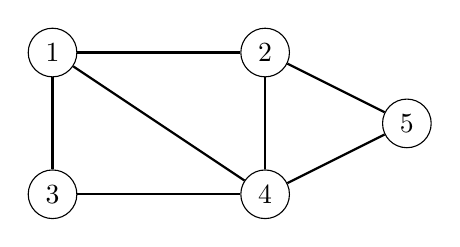
\begin{tikzpicture}[scale=0.9]
\node[draw, circle] (1) at (1,3) {$1$};
\node[draw, circle] (2) at (4,3) {$2$};
\node[draw, circle] (3) at (1,1) {$3$};
\node[draw, circle] (4) at (4,1) {$4$};
\node[draw, circle] (5) at (6,2) {$5$};

\path[draw,thick,-] (1) -- (2);
\path[draw,thick,-] (1) -- (3);
\path[draw,thick,-] (1) -- (4);
\path[draw,thick,-] (3) -- (4);
\path[draw,thick,-] (2) -- (4);
\path[draw,thick,-] (2) -- (5);
\path[draw,thick,-] (4) -- (5);
\end{tikzpicture}
\end{center}
một cách tô màu hợp lệ như sau:
\begin{center}
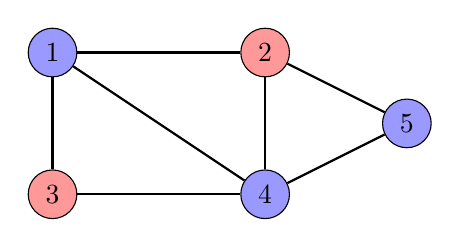
\begin{tikzpicture}[scale=0.9]
\node[draw, circle, fill=blue!40] (1) at (1,3) {$1$};
\node[draw, circle, fill=red!40] (2) at (4,3) {$2$};
\node[draw, circle, fill=red!40] (3) at (1,1) {$3$};
\node[draw, circle, fill=blue!40] (4) at (4,1) {$4$};
\node[draw, circle, fill=blue!40] (5) at (6,2) {$5$};

\path[draw,thick,-] (1) -- (2);
\path[draw,thick,-] (1) -- (3);
\path[draw,thick,-] (1) -- (4);
\path[draw,thick,-] (3) -- (4);
\path[draw,thick,-] (2) -- (4);
\path[draw,thick,-] (2) -- (5);
\path[draw,thick,-] (4) -- (5);
\end{tikzpicture}
\end{center}
Đồ thị trên chứa 7 cạnh, và với 5 trong số chúng,
các điểm cuối có màu khác nhau,
vì vậy việc tô màu là hợp lệ.

Bài toán có thể được giải quyết bằng một thuật toán Las Vegas
tạo ra các cách tô màu ngẫu nhiên cho đến khi một cách tô màu hợp lệ
được tìm thấy.
Trong một cách tô màu ngẫu nhiên, màu của mỗi nút được
chọn độc lập sao cho xác suất của
cả hai màu là $1/2$.

Trong một cách tô màu ngẫu nhiên, xác suất để các điểm cuối
của một cạnh đơn lẻ có màu khác nhau là $1/2$.
Do đó, số cạnh kỳ vọng có các điểm cuối
có màu khác nhau là $m/2$.
Vì kỳ vọng rằng một cách tô màu ngẫu nhiên là hợp lệ,
chúng ta sẽ nhanh chóng tìm thấy một cách tô màu hợp lệ trong thực tế.